%----------------------------------------------------------------------------------------
%	PACKAGES AND THEMES
%----------------------------------------------------------------------------------------
\documentclass[aspectratio=169,xcolor=dvipsnames]{beamer}

\definecolor{links}{HTML}{2A1B81}
\hypersetup{colorlinks,linkcolor=,urlcolor=links}

\usetheme{Berkeley}

\usepackage{xcolor}
\usepackage{hyperref}
\usepackage{graphicx} % Allows including images
\usepackage{booktabs} % Allows the use of \toprule, \midrule and \bottomrule in tables

%----------------------------------------------------------------------------------------
%	TITLE PAGE
%----------------------------------------------------------------------------------------

% The title
\title[Functional MRI: Part 1 of 2]{Understanding and Interpreting \\Functional Magnetic Resonance Imaging}
\subtitle{Precision Health Boot Camp}

\author[Dr. Alexander Mark Weber] {Alexander Mark Weber}
\institute[UBC] % Your institution may be shorthand to save space
{
    % Your institution for the title page
    Department of Pediatrics, Division of Neurology \\
    University of British Columbia 
    \vskip 3pt
}
\date{9:00 - 11:00 AM \\August 9th, 2022} % Date, can be changed to a custom date


%----------------------------------------------------------------------------------------
%	PRESENTATION SLIDES
%----------------------------------------------------------------------------------------

\begin{document}

\begin{frame}
    % Print the title page as the first slide
    \titlepage
\end{frame}

\begin{frame}{Preamble}

\begin{columns}[c]
\column{0.4\textwidth}
\begin{center}
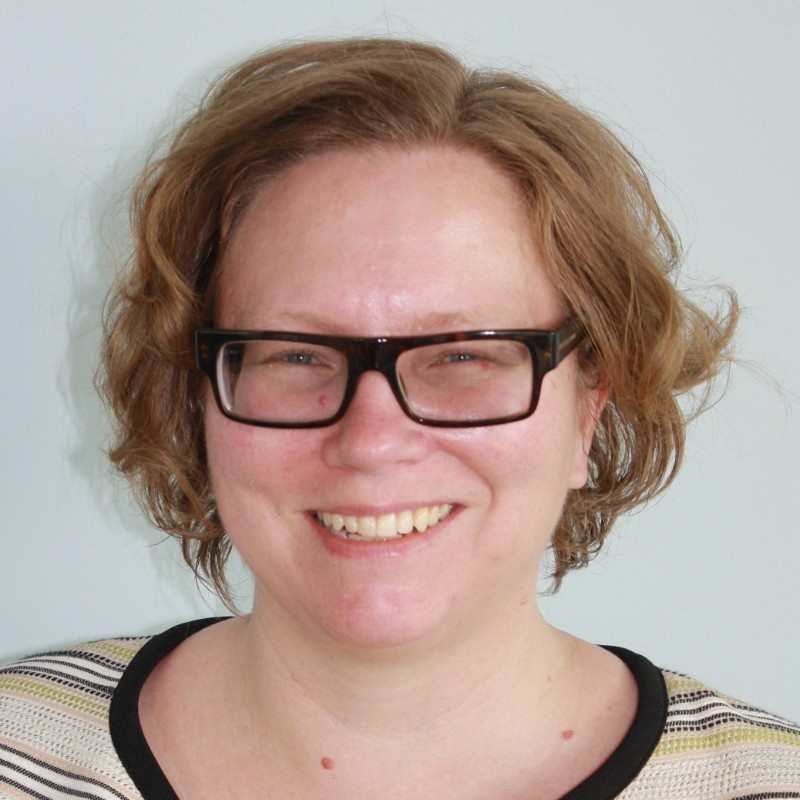
\includegraphics[width=.7\textwidth]{imgs/Lynne}
\end{center}

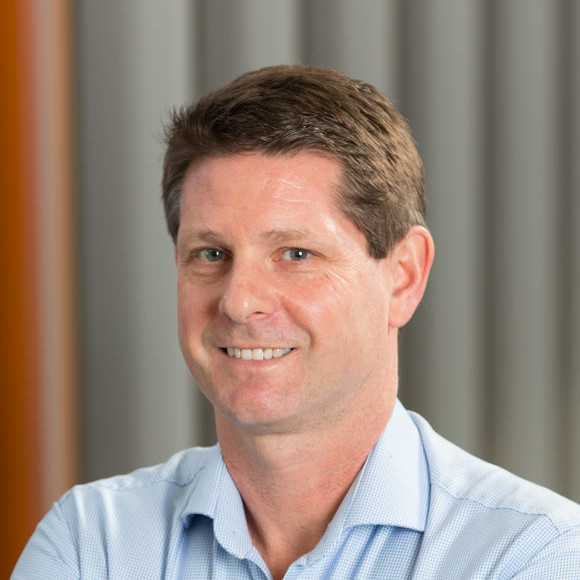
\includegraphics[width=.5\textwidth]{imgs/todd}%
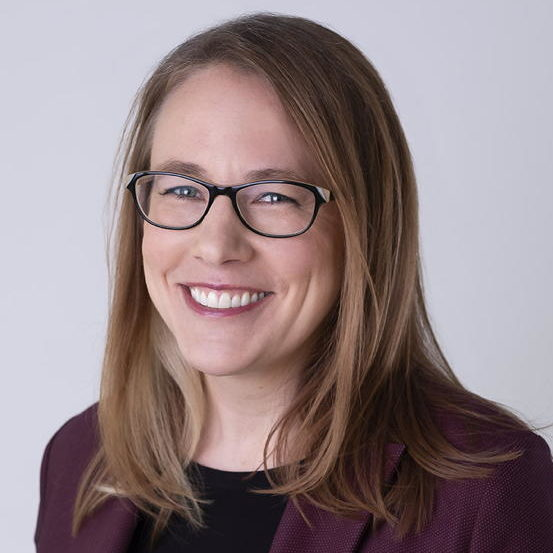
\includegraphics[width=.5\textwidth]{imgs/tammy}
\column{0.3\textwidth}

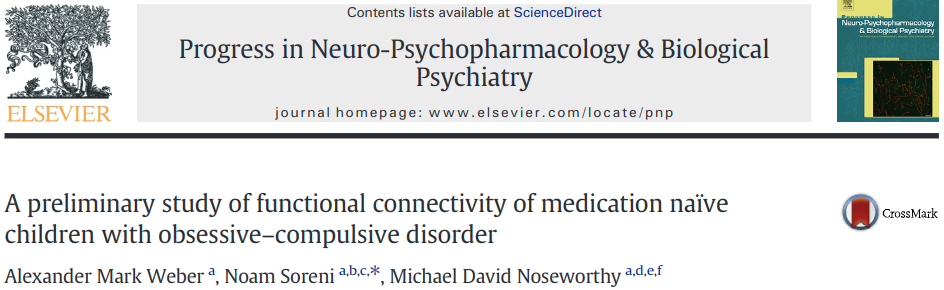
\includegraphics[width=1\textwidth]{imgs/lit1}

\vspace{1cm}

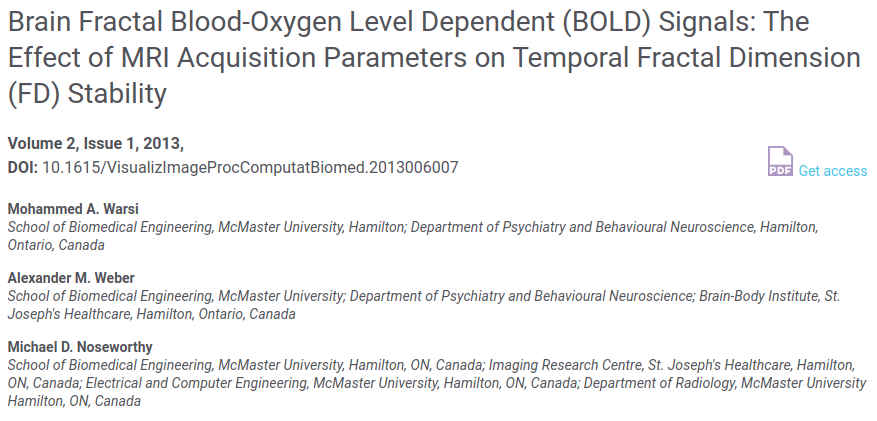
\includegraphics[width=1\textwidth]{imgs/lit3}

\vspace{1cm}


\includegraphics[width=1\textwidth]{imgs/lit5}

\column{0.3\textwidth}

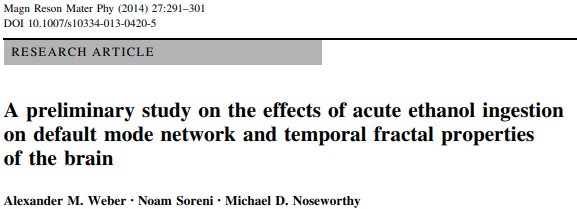
\includegraphics[width=1\textwidth]{imgs/lit2}

\vspace{1cm}

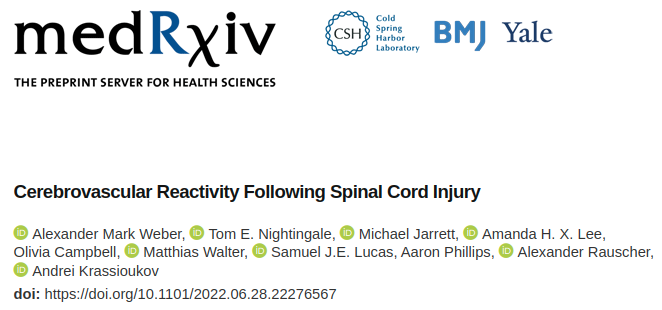
\includegraphics[width=1\textwidth]{imgs/lit4}

\end{columns}
\end{frame}

\begin{frame}{Overview}
    % Throughout your presentation, if you choose to use \section{} and \subsection{} commands, these will automatically be printed on this slide as an overview of your presentation
    \tableofcontents
\end{frame}

%------------------------------------------------
\section{Housekeeping}
%------------------------------------------------

\begin{frame}{Land Acknowledgement}

I would like to acknowledge that we are gathered today on the traditional, ancestral, and unceded territory of the Musqueam people.

\vspace{0.2cm}
\begin{center}
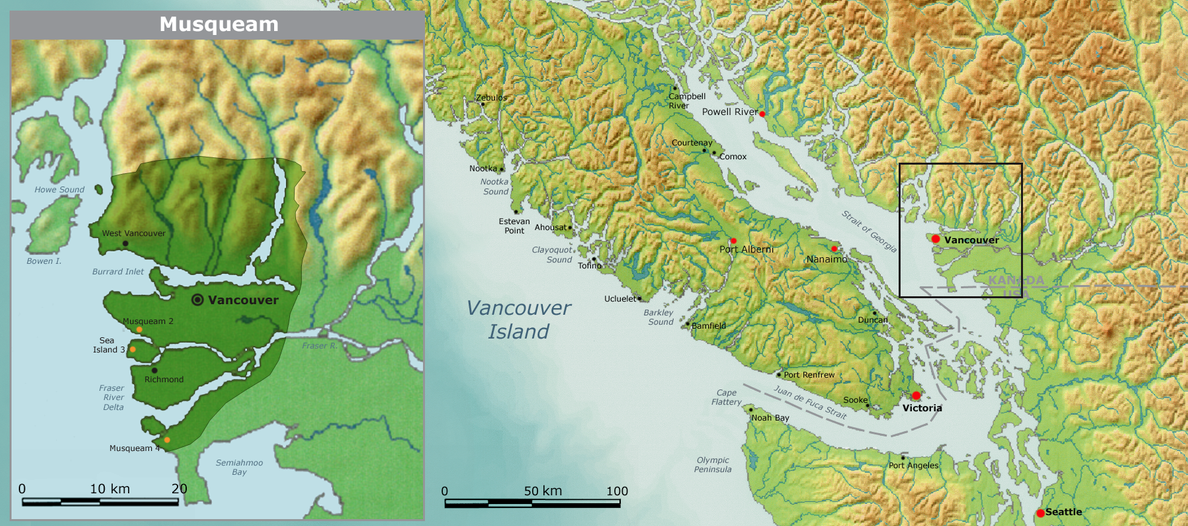
\includegraphics[width=.9\textwidth]{imgs/musqueam}
\end{center}

\end{frame}

%------------------------------------------------

\begin{frame}{Copyright Information}

\begin{columns}[c]
\column{0.5\textwidth}
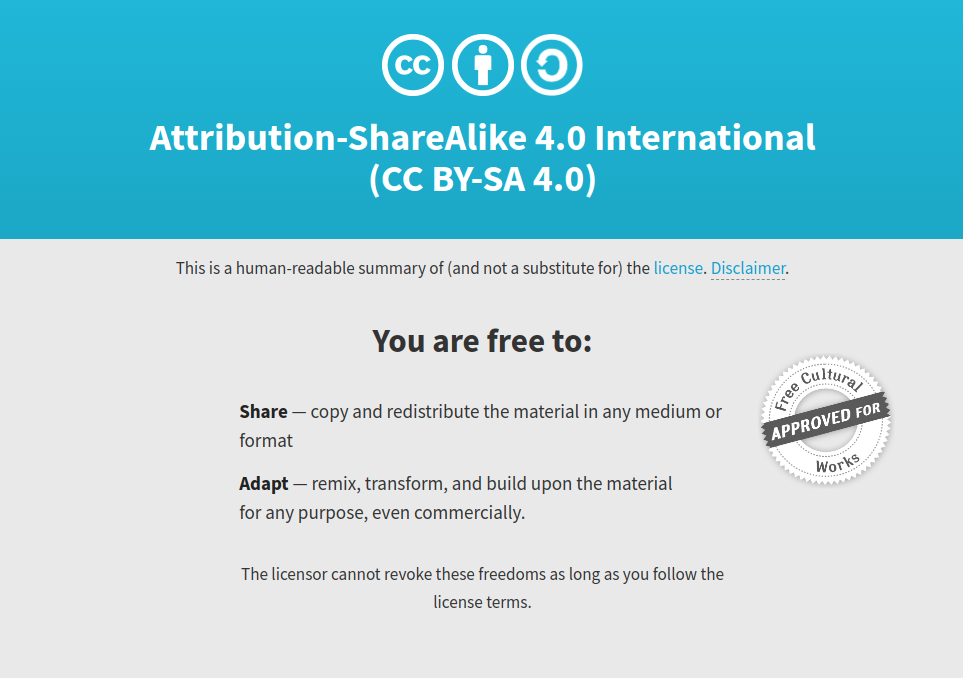
\includegraphics[width=1\textwidth]{imgs/cc}
\column{0.5\textwidth}
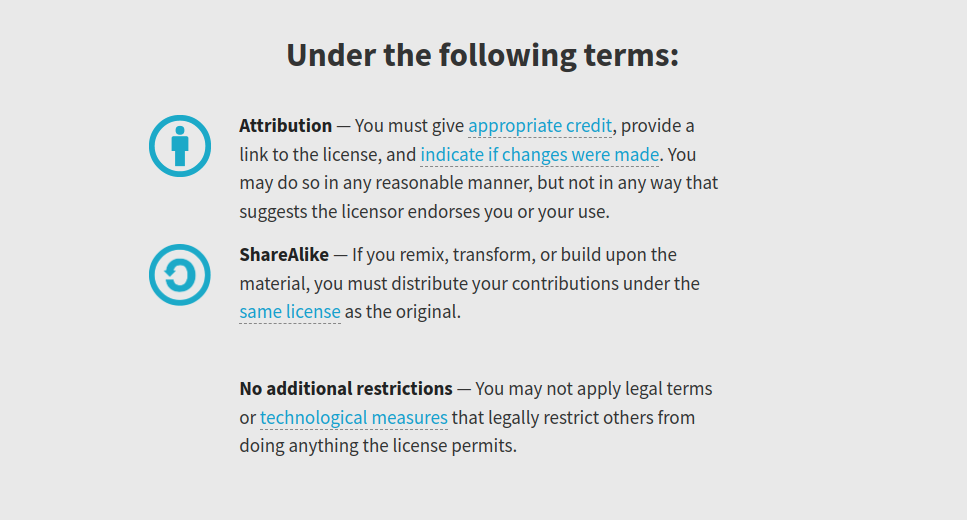
\includegraphics[width=1\textwidth]{imgs/cc2}
\end{columns}

\vspace{.5cm}
Read more here: \url{https://creativecommons.org/licenses/by-sa/4.0/}

\end{frame}

%------------------------------------------------
\section{fMRI Overview}
%------------------------------------------------

\begin{frame}{fMRI Overview}
\begin{columns}[c]
\column{0.3\textwidth}
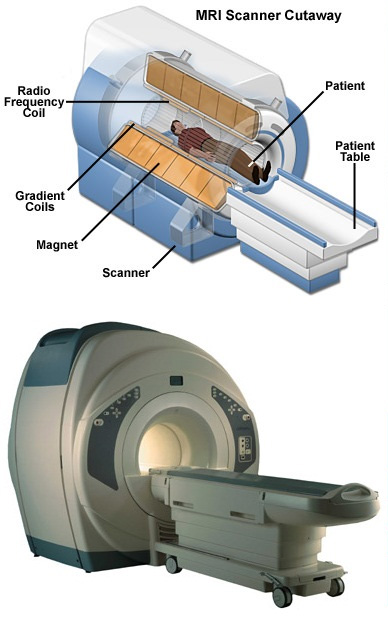
\includegraphics[width=1\textwidth]{imgs/MRI}
\tiny{https://www.northwestradiology.com/blog/page/16/}
\column{0.7\textwidth}
\begin{itemize}
\item \textbf{Magnetic:} Large magnet: 1.5 Tesla to 10 Tesla strength
\item Earth's magnetic field is 0.00005 Tesla
\item Our BCCHR Research MRI is 3T; ~ 60,000x Earth's magnetic field
\item \textbf{Resonance:} Uses radiowaves with frequencies that resonate with atomic nuclei (hydrogen, usually)
\item \textbf{Imaging:} Converts spatial frequencies and phase into images
\end{itemize}
\end{columns}
\end{frame}

%------------------------------------------------

\begin{frame}{fMRI Overview}
\begin{columns}[c]
\column<1->{0.45\textwidth}
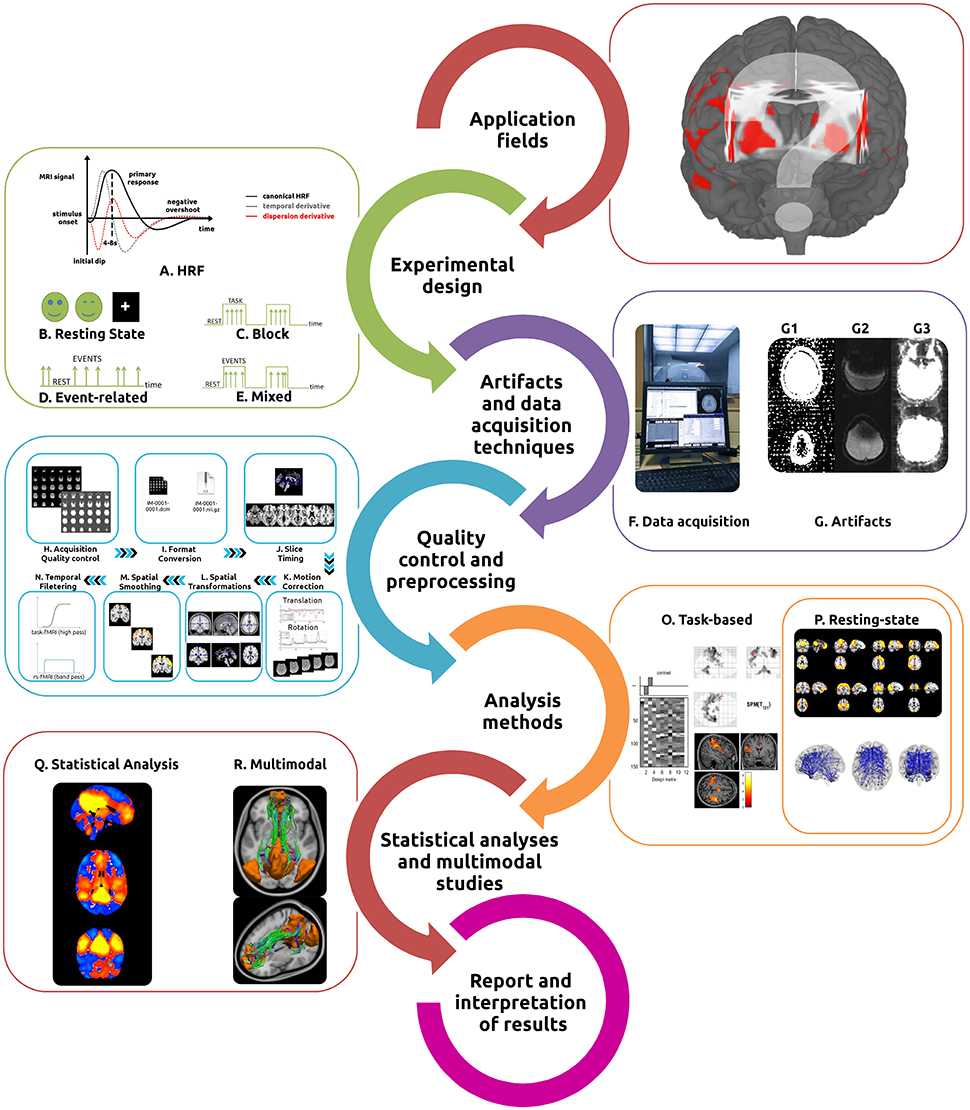
\includegraphics[width=1\textwidth]{imgs/fmri_overview}
\tiny{Soares et al. (2016) Front Neurosci, 10(515)}

\column<2->{0.55\textwidth}
Lecture:
\begin{itemize}
\item MRI Physics
\item Brain physiology
\item fMRI acquisition
\item Task vs Resting State fMRI
\end{itemize}

Tutorial:
\begin{itemize}
\item Get data from PACS; Copy over to Sockeye
\item Conversion and preprocessing (two ways)
\item Nuisance regression (two ways)
\end{itemize}
\end{columns}

\end{frame}

%------------------------------------------------
\section{MRI Physics}
%------------------------------------------------

\begin{frame}{MRI Physics Overview}
\begin{columns}[c]
\column{0.33\textwidth}
\includegraphics<1->[width=1\textwidth]{imgs/planet}
\column{0.33\textwidth}
\includegraphics<2->[width=1\textwidth]{imgs/gyro-0}
\column{0.33\textwidth}
\includegraphics<3->[width=1\textwidth]{imgs/protoncharge}
\end{columns}
\end{frame}

%------------------------------------------------

\begin{frame}{MRI Physics Overview}
\begin{columns}[c]
\column{0.33\textwidth}
\includegraphics<1->[width=1\textwidth]{imgs/magnet}
\column{0.33\textwidth}
\includegraphics<2->[width=1\textwidth]{imgs/extmagfield}
\column{0.33\textwidth}
\includegraphics<3->[width=1\textwidth]{imgs/precession}
\end{columns}
\end{frame}

%------------------------------------------------

\begin{frame}{MRI Physics Overview}
\begin{columns}[c]
\column{0.33\textwidth}
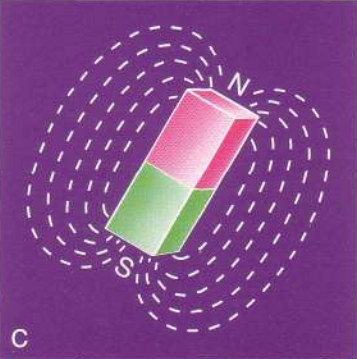
\includegraphics[width=1\textwidth]{imgs/magnet}
\column{0.33\textwidth}
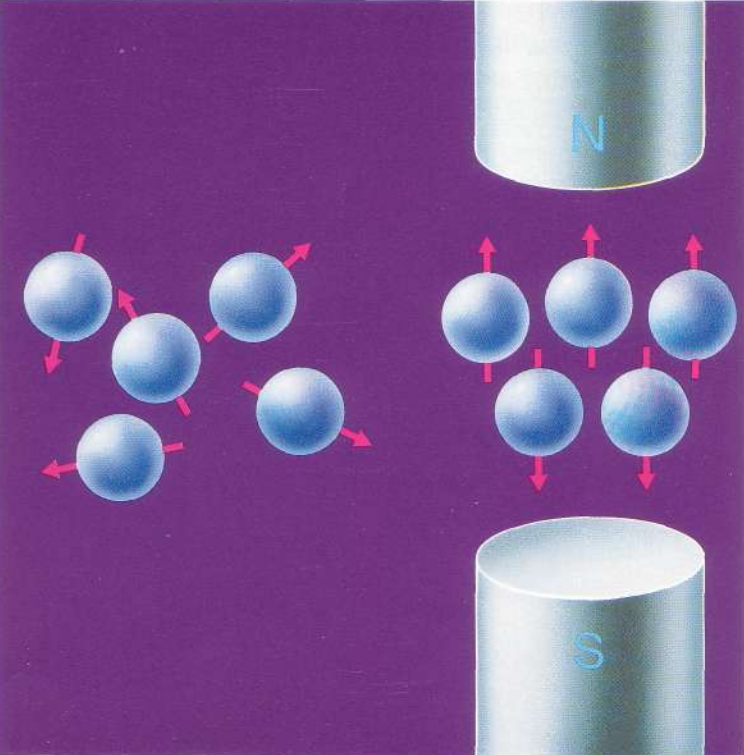
\includegraphics[width=1\textwidth]{imgs/extmagfield}
\column{0.33\textwidth}
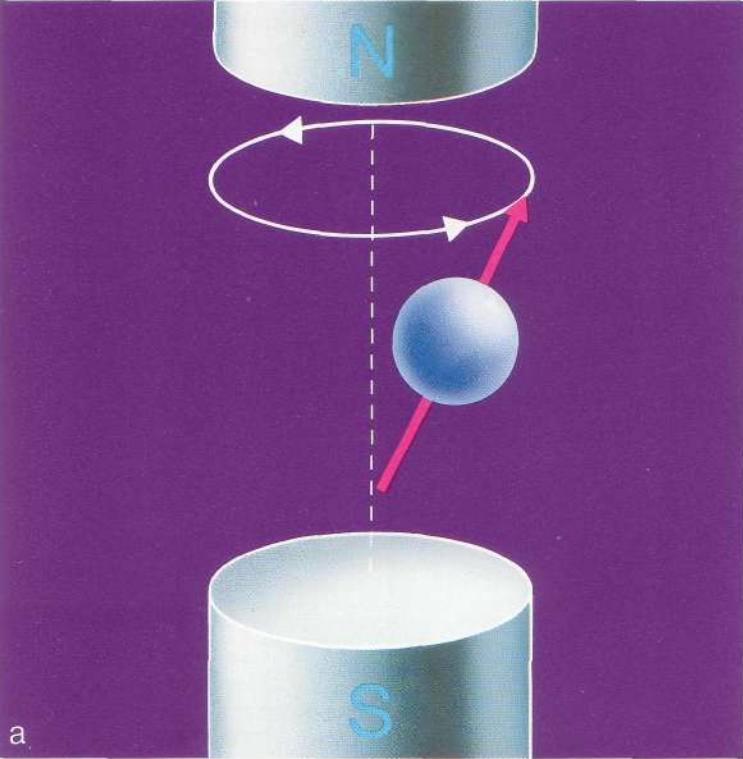
\includegraphics[width=1\textwidth]{imgs/precession2}
\end{columns}
\end{frame}

%------------------------------------------------

\begin{frame}{MRI Physics Overview}
\begin{columns}[c]
\column{0.6\textwidth}
\includegraphics<1->[width=1\textwidth]{imgs/cancel}
\column{0.4\textwidth}
\includegraphics<2->[width=1\textwidth]{imgs/cancel2}
\end{columns}
\end{frame}

%------------------------------------------------

\begin{frame}{MRI Physics Overview}
\begin{center}
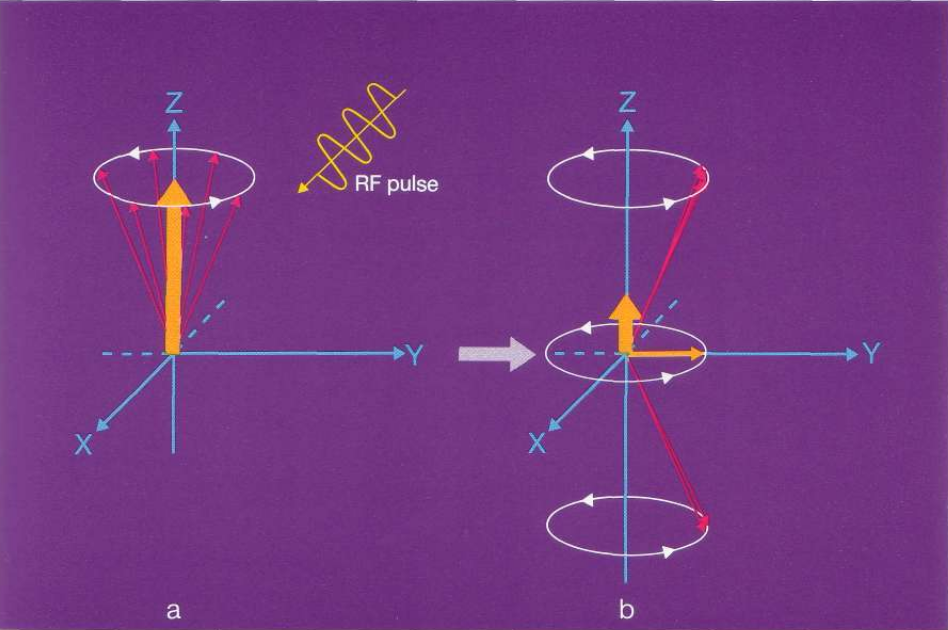
\includegraphics[width=.6\textwidth]{imgs/rfpulse}

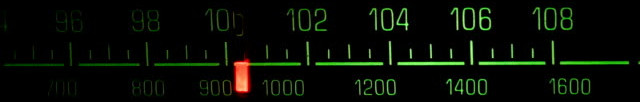
\includegraphics[width=.6\textwidth]{imgs/fmdial}
\end{center}
\end{frame}

%------------------------------------------------

\begin{frame}{MRI Physics Overview}
\begin{center}
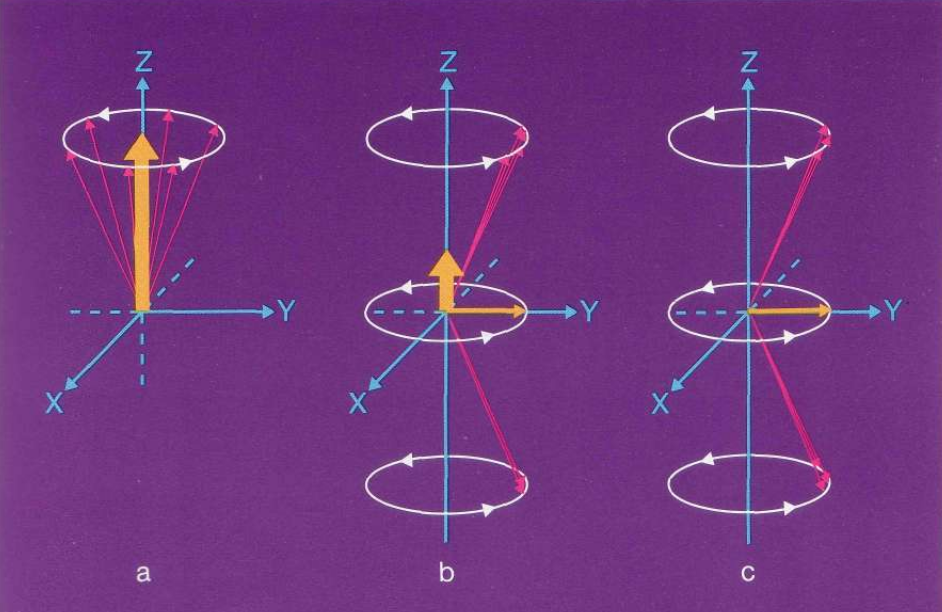
\includegraphics[width=.75\textwidth]{imgs/rfpulse2}

\end{center}
\end{frame}

%------------------------------------------------

\begin{frame}{MRI Physics Overview}
\begin{columns}[c]
\column{0.5\textwidth}
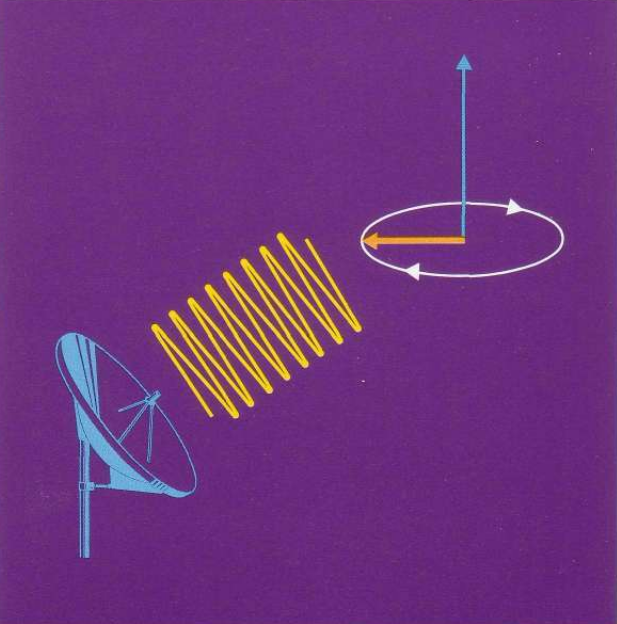
\includegraphics[width=1\textwidth]{imgs/rfpulse3}
\column{0.5\textwidth}
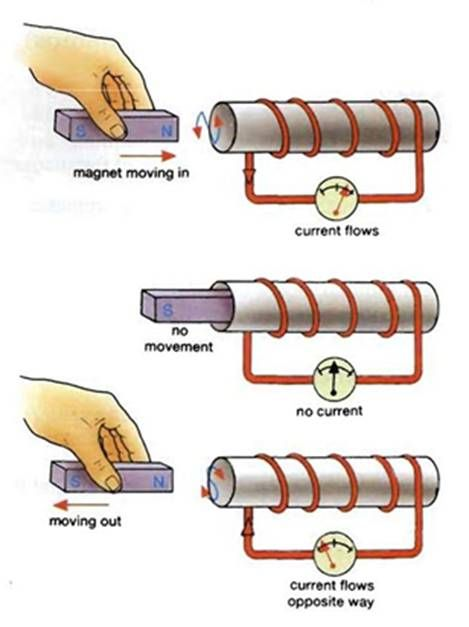
\includegraphics[width=.7\textwidth]{imgs/faradaylaw}
\end{columns}
\end{frame}

%------------------------------------------------

\begin{frame}{MRI Physics Summary}

\begin{itemize}
\item Proton's have QM Spin
\item When placed in a large magnet (MRI) these protons precess around the main magnetic field
\item Some face up and others face down, many cancelling each other out
\item If we send a RF pulse at the same precession frequency, we can put these protons in phase: we create a transverse magnetic field, and destroy the longitudinal one
\item This transverse magnetic field can be measured thanks to Faraday's Law of Induction
\end{itemize}

\end{frame}

%------------------------------------------------

\begin{frame}{T$_{2}^{*}$ Overview}
\begin{columns}[c]
\column{0.35\textwidth}
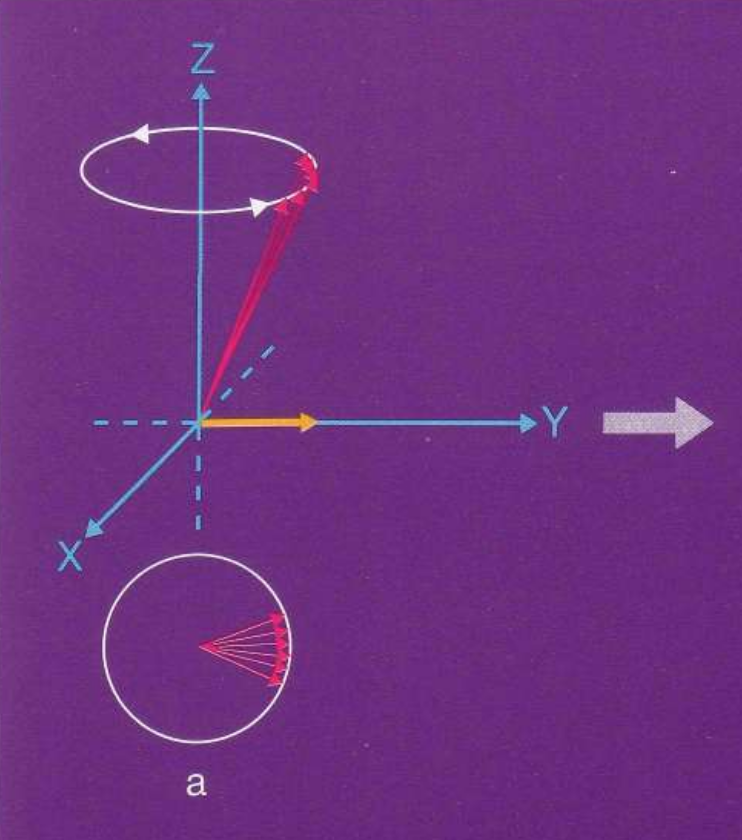
\includegraphics[width=1\textwidth]{imgs/transrelax}
\column{0.65\textwidth}
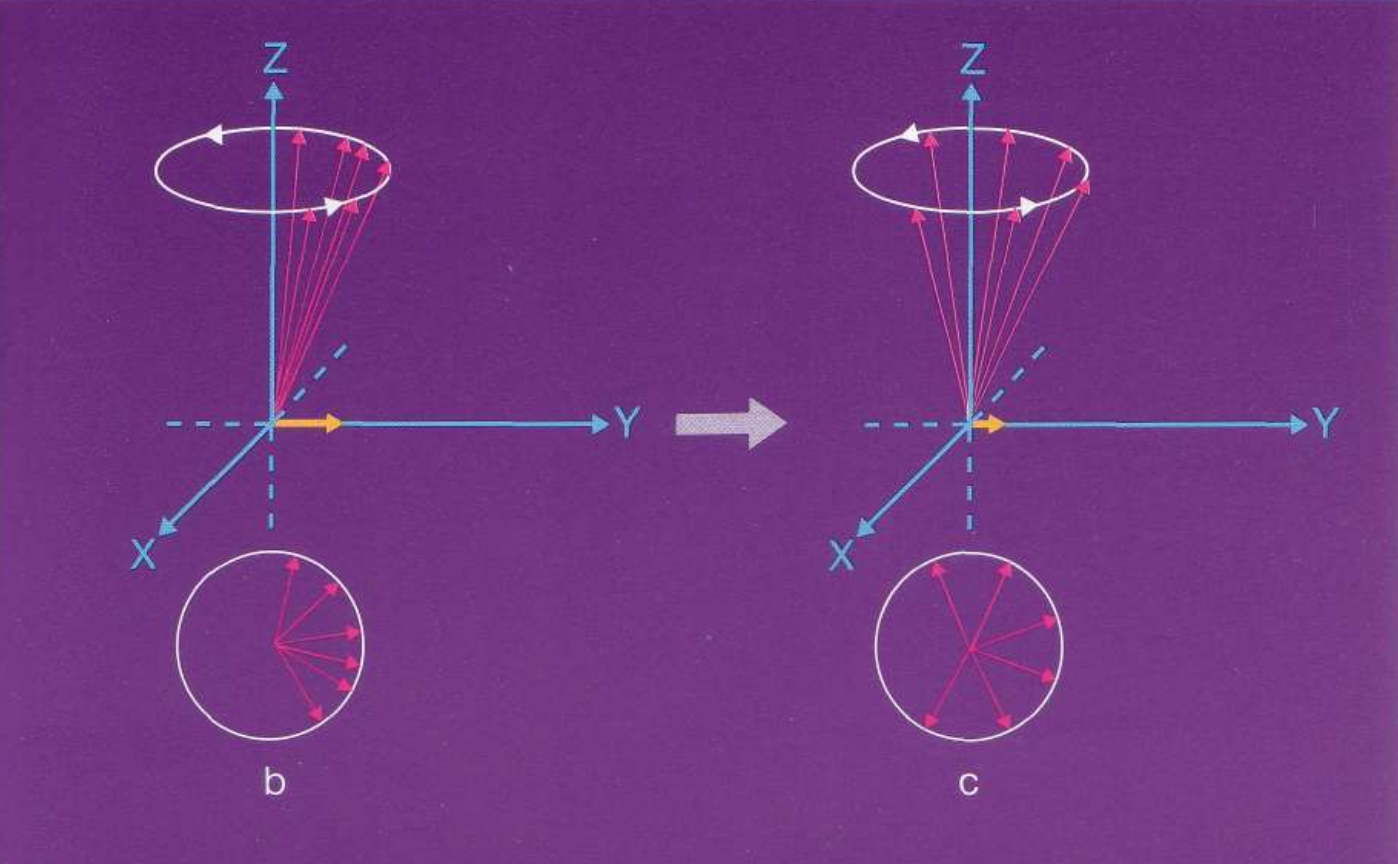
\includegraphics[width=1\textwidth]{imgs/transrelax2}
\end{columns}

\end{frame}

%------------------------------------------------

\begin{frame}{T$_{2}^{*}$ Overview}
    \begin{block}{T2 relaxation}
        Also known as spin-spin decay: it is a time measure of the rate of decay caused by spin-spin interactions
    \end{block}
\begin{center}
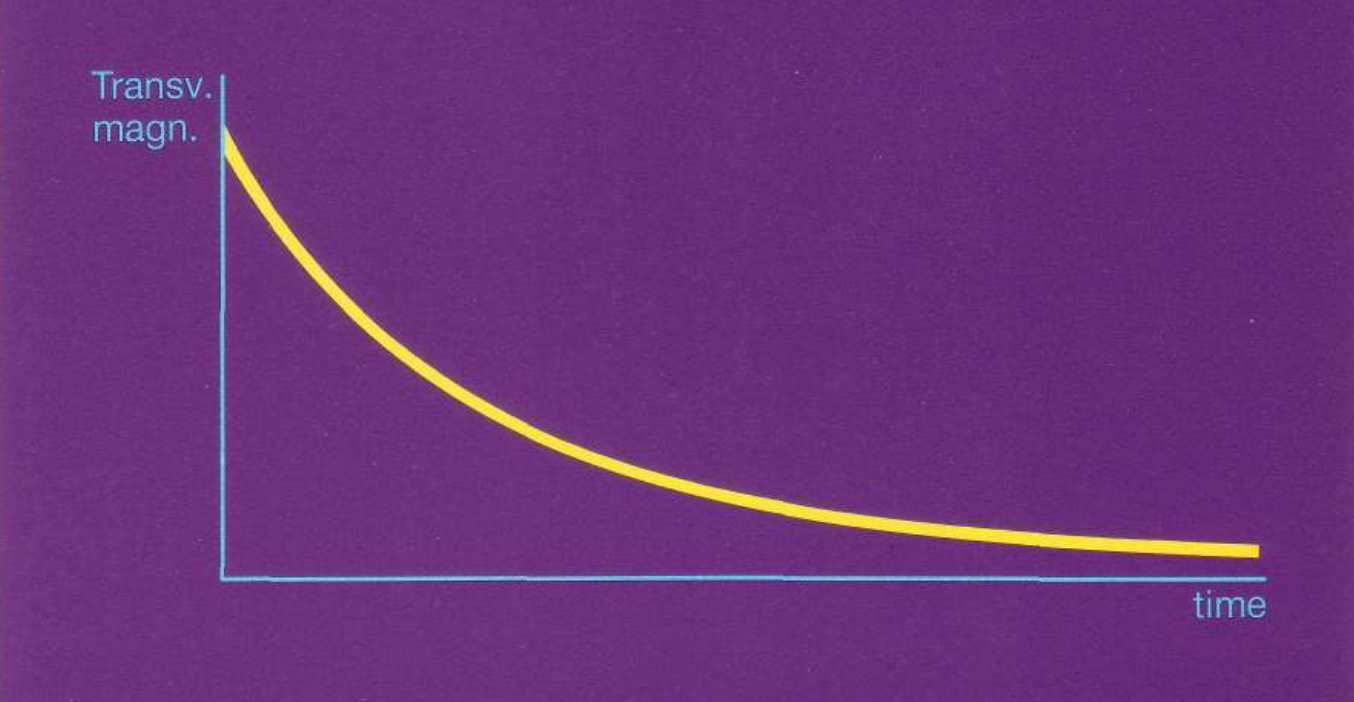
\includegraphics[width=.75\textwidth]{imgs/T2curv}

\end{center}
\end{frame}

%------------------------------------------------

\begin{frame}{T$_{2}^{*}$ Overview}
\begin{columns}[c]
\column<1->{0.5\textwidth}
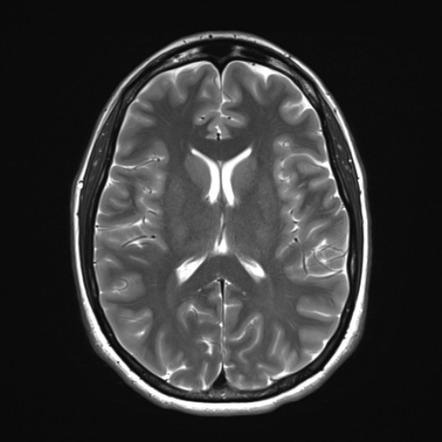
\includegraphics[width=1\textwidth]{imgs/t2brain}
\column<2->{0.5\textwidth}
T$_{2}$-weighted scan
\begin{itemize}
\item Water is bright
\item A mix of water/tissue is less bright (grey matter)
\item Fatty tissue is dark (white matter)
\end{itemize}
\end{columns}

\end{frame}

%------------------------------------------------

\begin{frame}{T$_{2}^{*}$ Overview}

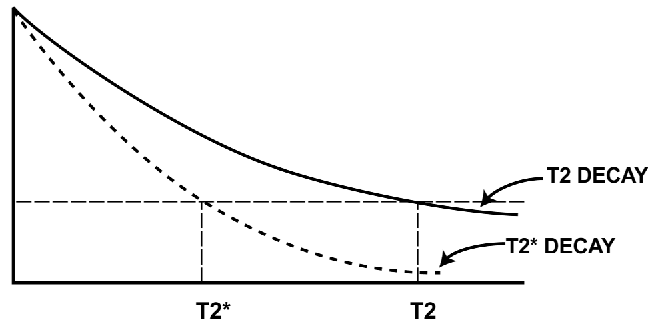
\includegraphics[width=1\textwidth]{imgs/t2stardecay}

\tiny{Chavhan et al. DOI: 10.1148/rg.295095034}

\end{frame}

%------------------------------------------------

\begin{frame}{T$_{2}^{*}$ Overview}
\begin{columns}[c]
\column<1->{0.5\textwidth}
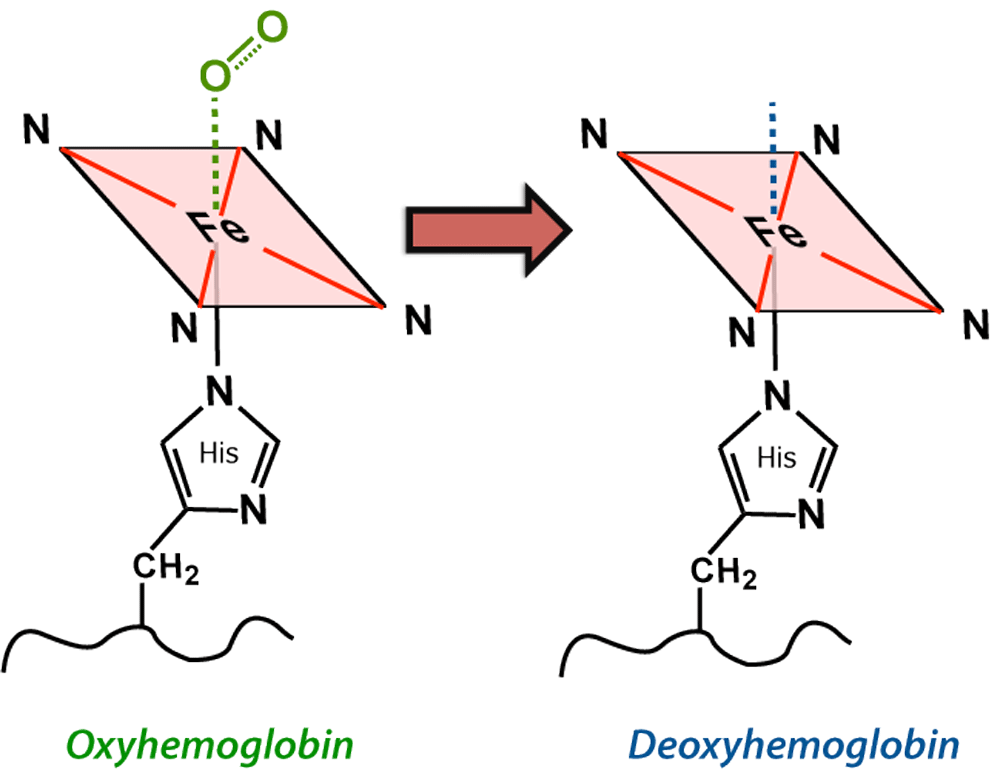
\includegraphics[width=1\textwidth]{imgs/deoxy}
\column<2->{0.5\textwidth}
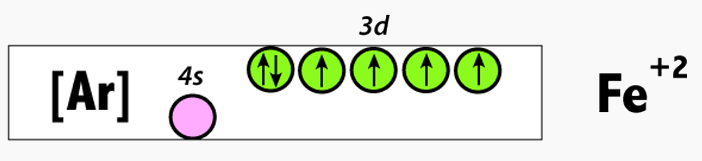
\includegraphics[width=1\textwidth]{imgs/ferrous}
\end{columns}

\end{frame}

%------------------------------------------------
\section{BOLD Effect}
%------------------------------------------------

\begin{frame}{Neurovascular Coupling}

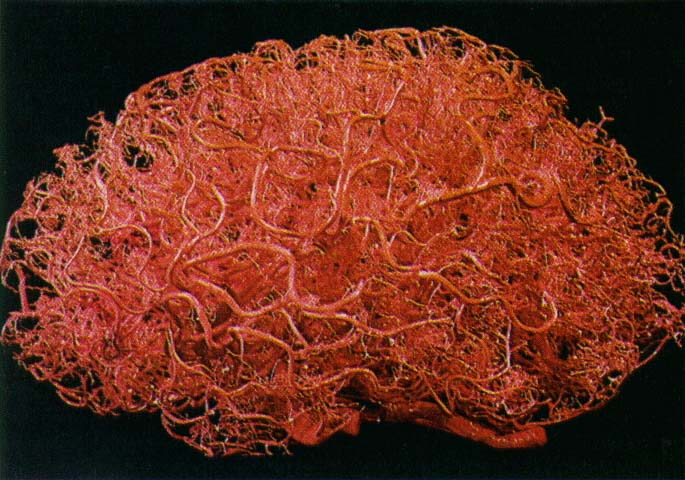
\includegraphics[width=.7\textwidth]{imgs/brainveins}

\tiny{Zlokovic, B. and Apuzzo, M. (1998). Strategies to Circumvent Vascular Barriers of the Central Nervous System. Neurosurgery 43, 877-878.}
\end{frame}

%------------------------------------------------

\begin{frame}{Neurovascular Coupling}

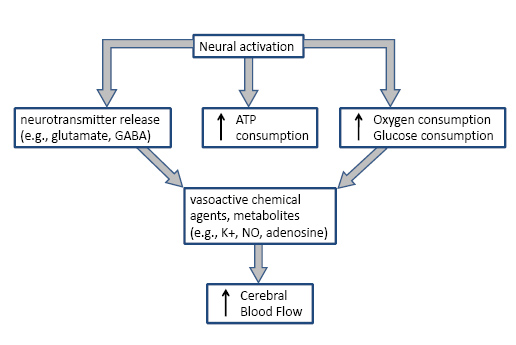
\includegraphics[width=.75\textwidth]{imgs/neurovasccoupling}

\end{frame}

%------------------------------------------------

\begin{frame}{Neurovascular Coupling}

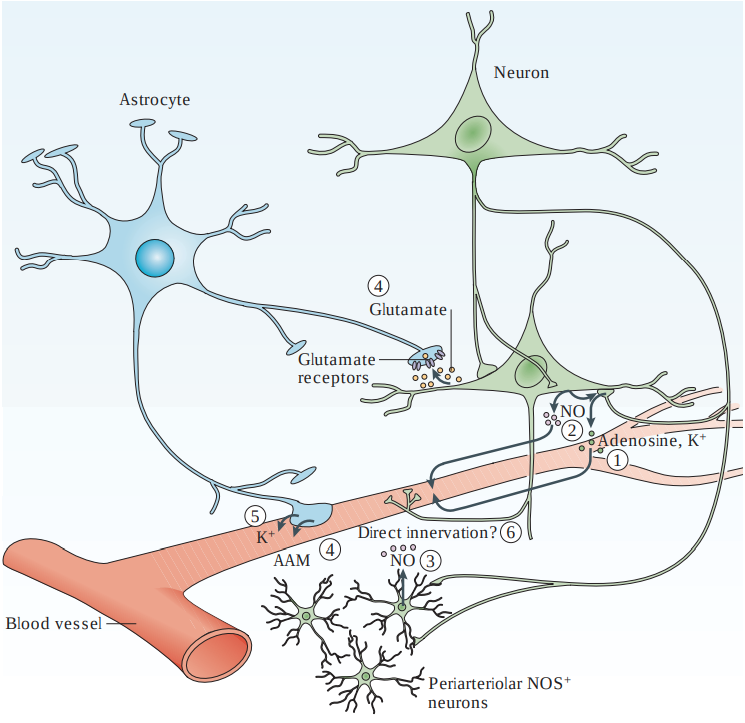
\includegraphics[width=.5\textwidth]{imgs/neurovasc3}

\tiny{D’Esposito et al. (2003). Nature Reviews Neuroscience, 4}
\end{frame}

%------------------------------------------------

\begin{frame}{BOLD Effect}
\begin{columns}[c]
\column<1->{0.5\textwidth}
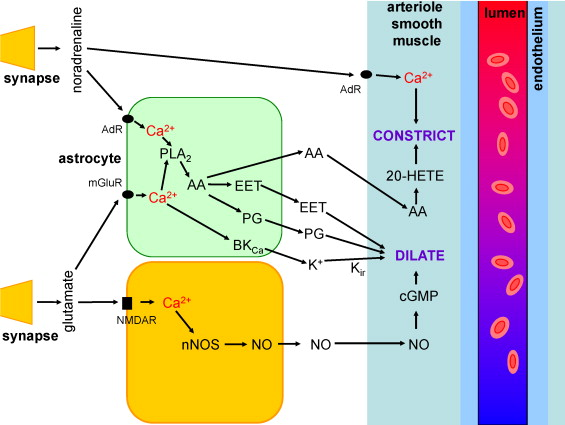
\includegraphics[width=1\textwidth]{imgs/neurovasccoupling2}
\column<2->{0.5\textwidth}
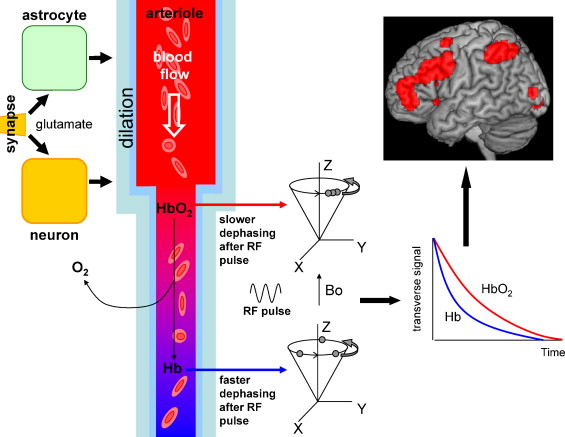
\includegraphics[width=1\textwidth]{imgs/bold}
\end{columns}

\tiny{Harris et al.  (2011). Developmental Cognitive Neuroscience, 1, 3}
\end{frame}

%------------------------------------------------

\begin{frame}{BOLD Effect}
\begin{columns}[c]
\column<1->{0.5\textwidth}
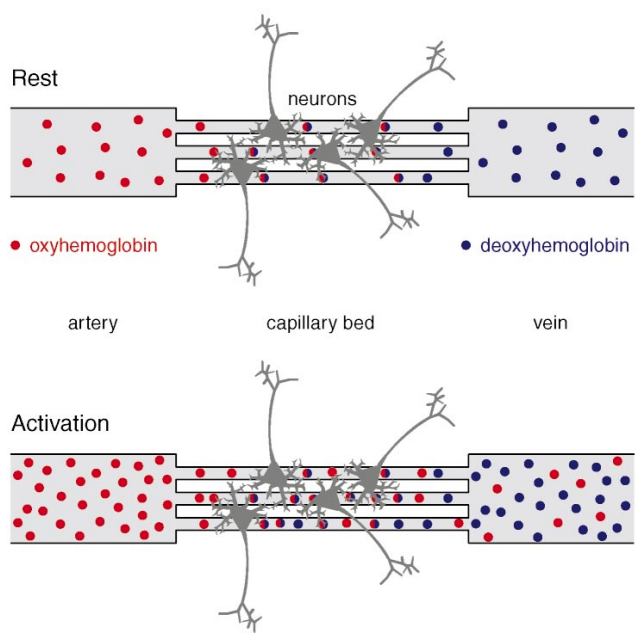
\includegraphics[width=1\textwidth]{imgs/BOLDeffect}
\tiny{Dogil et al. (2002). Journal of Neurolinguistics, 15(1), 59-90}
\column<1->{0.5\textwidth}
\begin{itemize}
\item<1-> Under normal conditions, \textcolor{red}{oxygenated hemoglobin} is converted to \textcolor{blue}{deoxygenated hemoglobin} within the capillary bed at a constant rate
\item<2-> When neurons become \textbf{active}, the vascular system supplies more \textcolor{red}{oxygenated hemoglobin} than is needed via an overcompensatory increase in blood flow.
\item<3-> The result is a net \textbf{decrease} in \textcolor{red}{deoxygenated hemoglobin} and a corresponding \textbf{decrease in signal loss} due to T$_{2}^{*}$ effects
\end{itemize}
\end{columns}
\end{frame}

%------------------------------------------------

\begin{frame}{Hemodynamic Response Function}

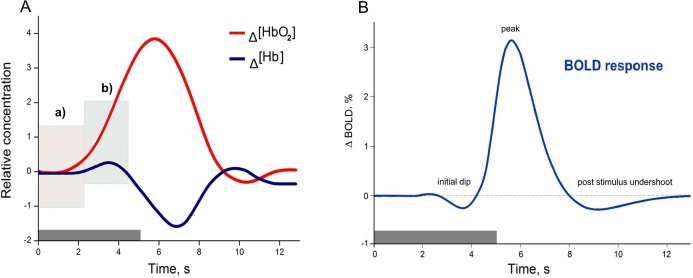
\includegraphics[width=1\textwidth]{imgs/HRF}
\tiny{Sigita Cinciute (2019) PeerJ, Mar 25;7e6621}

\normalsize{[Note: Please see work by Todd Woodward and others about how this shape should \textbf{NOT} be assumed]}
\end{frame}

%------------------------------------------------
\section{fMRI Acquisition}
%------------------------------------------------

\begin{frame}{fMRI Acquisition}
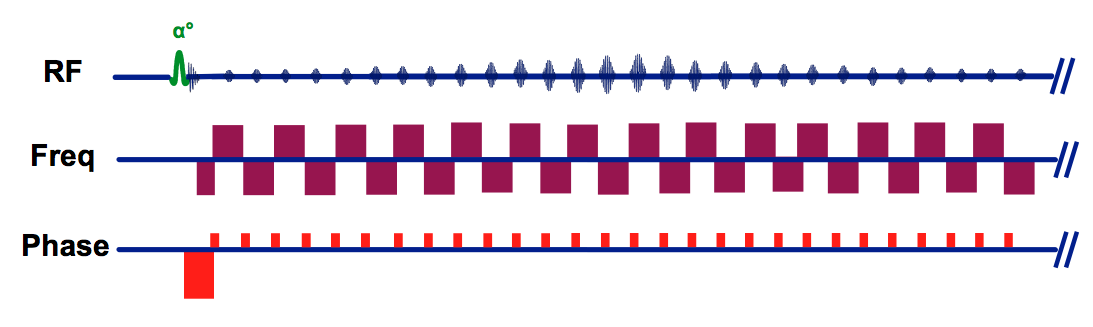
\includegraphics[width=.8\textwidth]{imgs/epipulsesignal}

\begin{center}
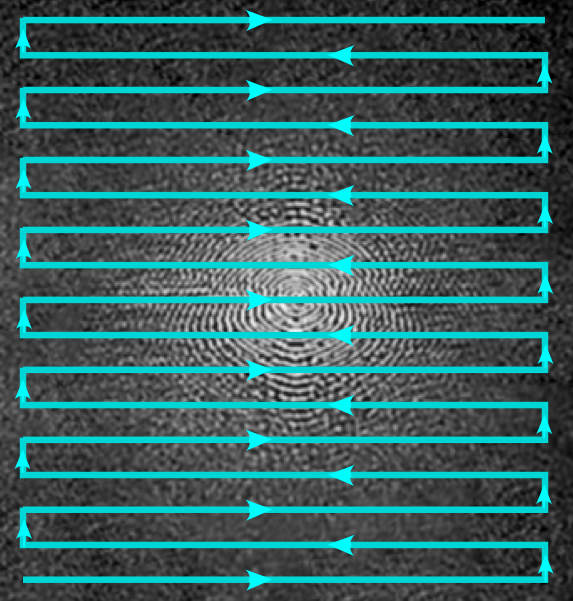
\includegraphics[width=.25\textwidth]{imgs/epikspace}
\end{center}

\tiny{https://mriquestions.com/echo-planar-imaging.html}
\end{frame}

%------------------------------------------------

\begin{frame}{fMRI Acquisition}
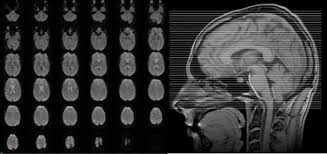
\includegraphics[width=1\textwidth]{imgs/fmrislices}
\end{frame}

%------------------------------------------------

\begin{frame}{fMRI Acquisition}
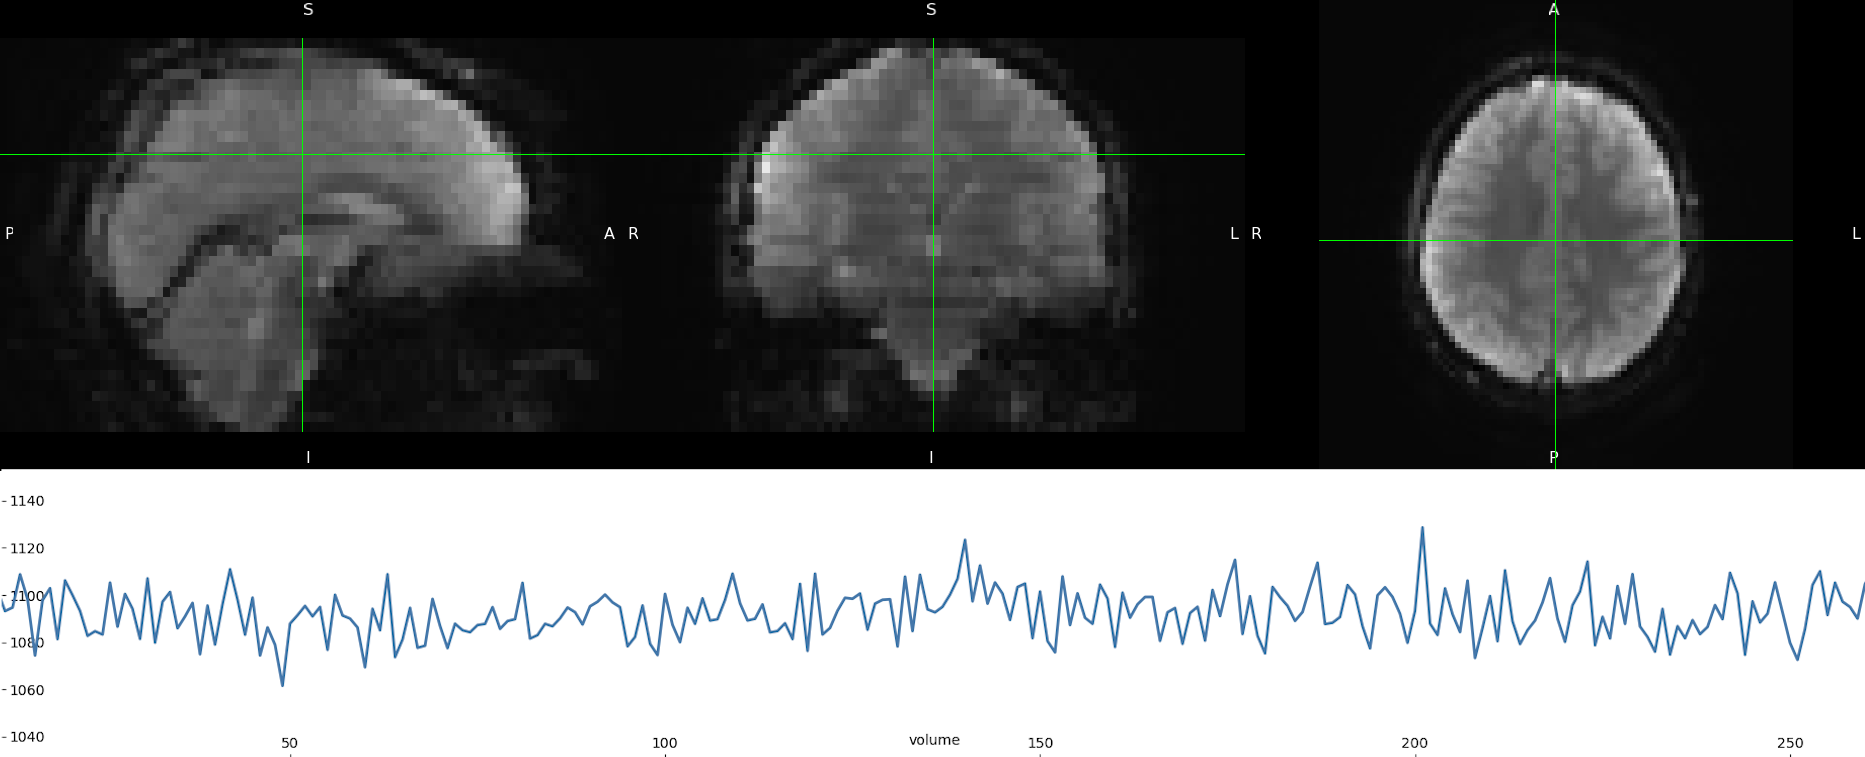
\includegraphics[width=1\textwidth]{imgs/fmritimeseries}
\end{frame}

%------------------------------------------------

\begin{frame}{fMRI Acquisition: Task-based}

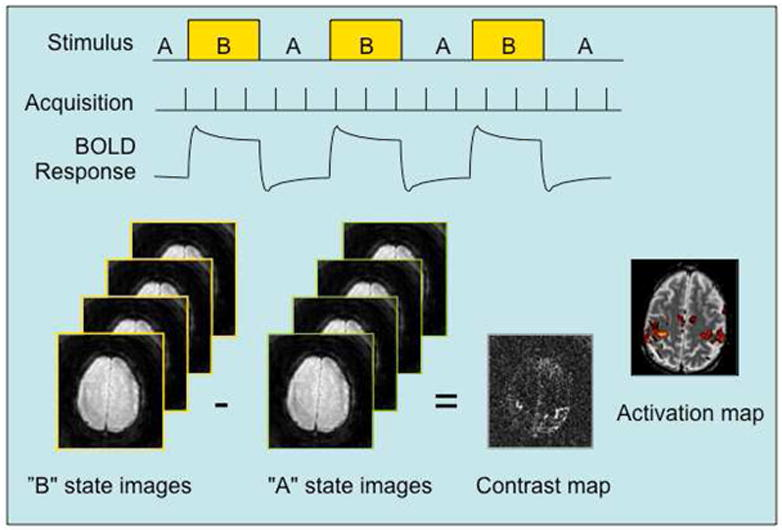
\includegraphics[width=.7\textwidth]{imgs/taskfmri}

\tiny{Gary Glover. (2011). Neurosurg Clin N Am, 22(2): 133-139}
\end{frame}

%------------------------------------------------

\begin{frame}{fMRI Acquisition: Task-based}
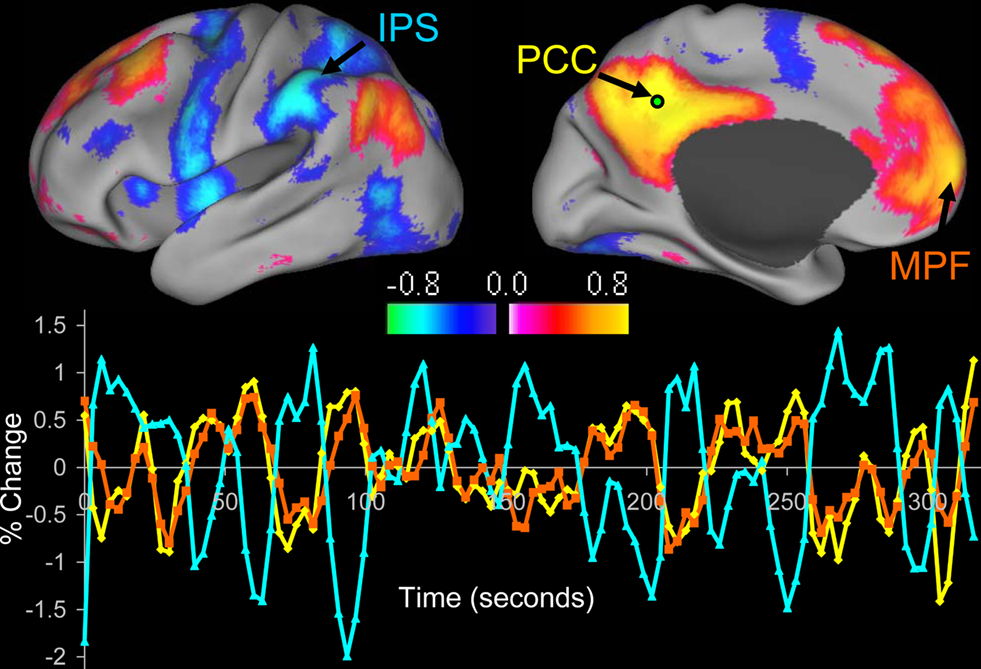
\includegraphics[width=.7\textwidth]{imgs/restingfmri}

\tiny{Fox and Greicius. (2010). Front Syst Neurosci, 4(19)}
\end{frame}

%------------------------------------------------
\section{fMRI Analysis}
%------------------------------------------------

\begin{frame}{fMRI Analysis: Preprocessing}
\begin{columns}[c]
\column<1->{0.7\textwidth}
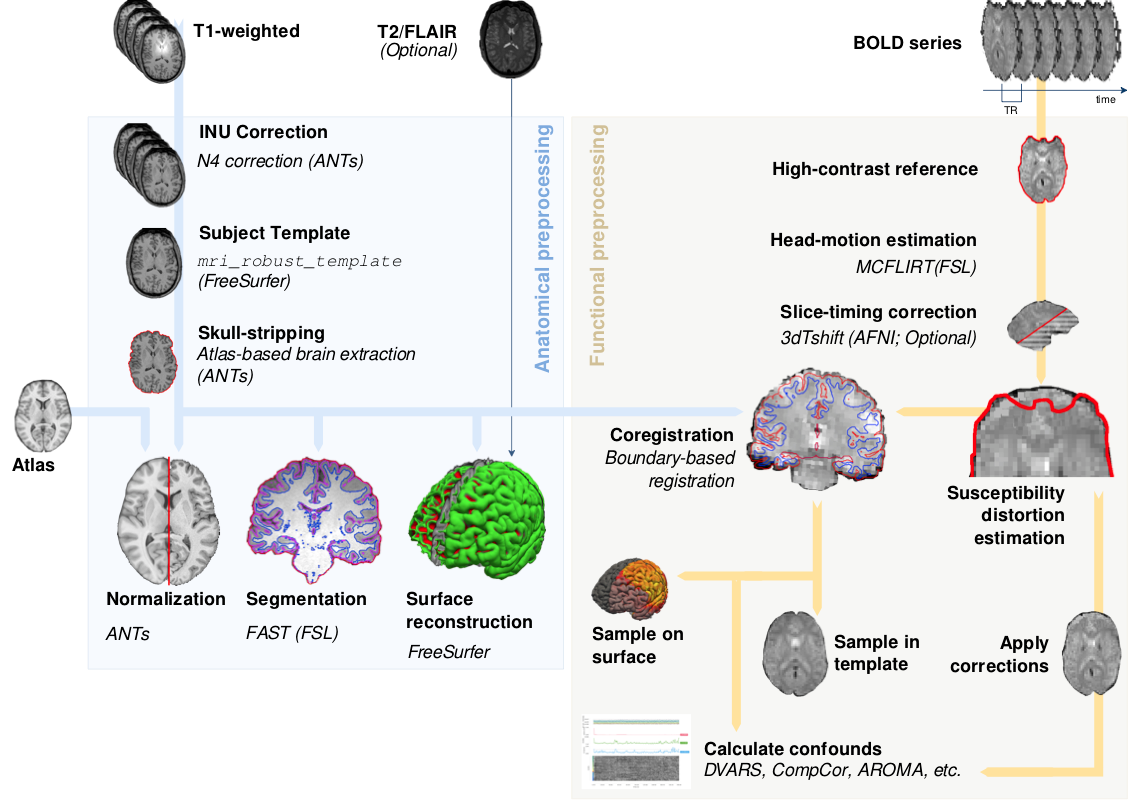
\includegraphics[width=1\textwidth]{imgs/preprocess}

\tiny{Markiewicz et al. (2018). OHBM Poster \#2305}

\column<2->{0.3\textwidth}
\begin{itemize}
\item Brain extraction
\item Motion correction
\item Slice-timing correction
\item Susceptibility distortion correction
\item Registration and Normalization
\item Estimate noise/confounds
\item Data quality check
\end{itemize}
\end{columns}
\end{frame}

%------------------------------------------------

\begin{frame}{fMRI Analysis: Preprocessing}

\url{https://openneuro.org/}

\vspace{0.2cm}
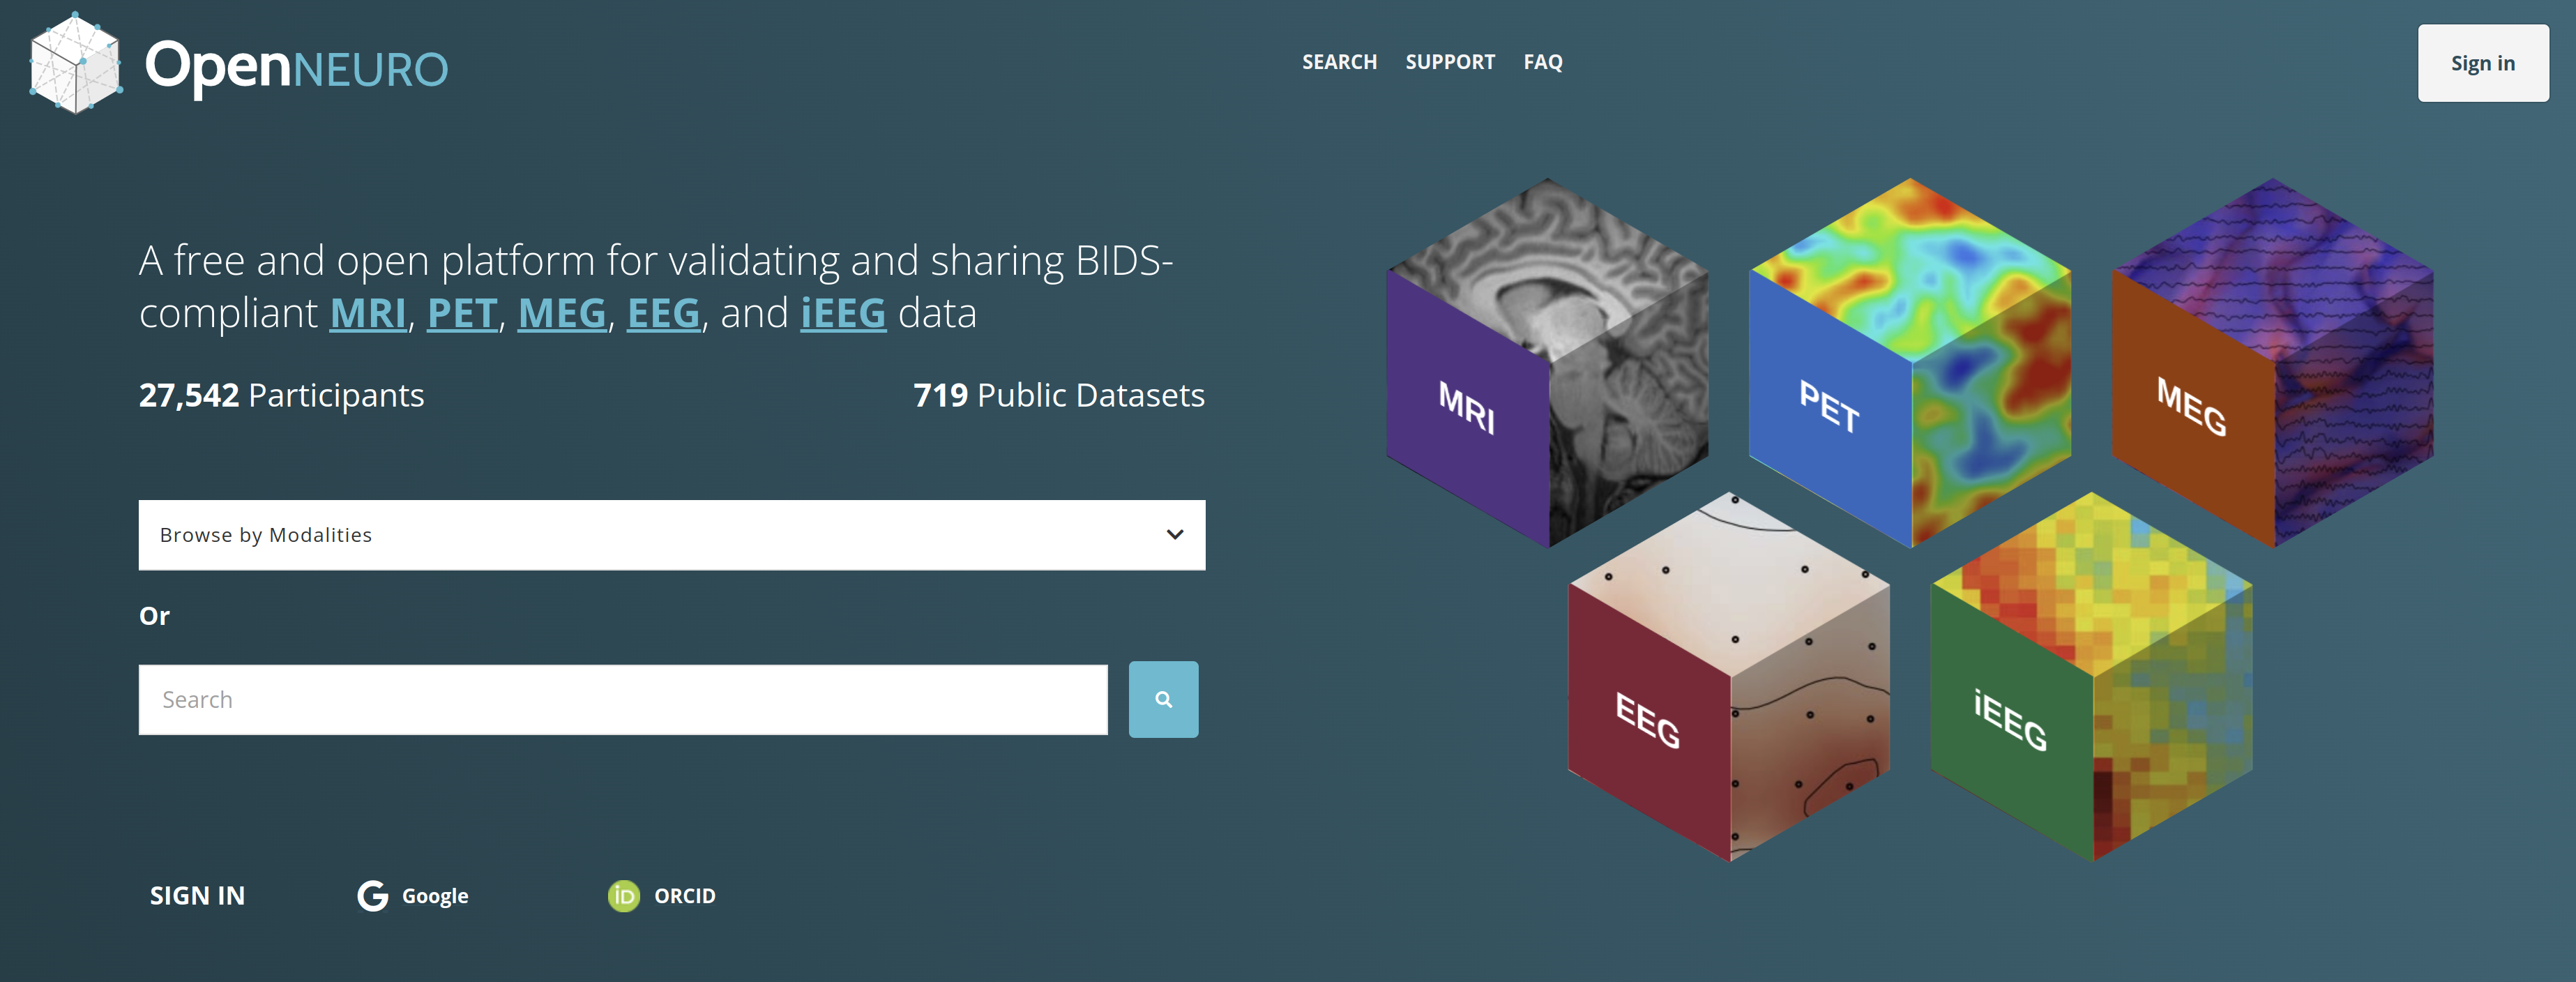
\includegraphics[width=1\textwidth]{imgs/openneuro}

\end{frame}

%------------------------------------------------




\begin{frame}{Blocks of Highlighted Text}
    In this slide, some important text will be \alert{highlighted} because it's important. Please, don't abuse it.

    \begin{block}{Block}
        Sample text
    \end{block}

    \begin{alertblock}{Alertblock}
        Sample text in red box
    \end{alertblock}

    \begin{examples}
        Sample text in green box. The title of the block is ``Examples".
    \end{examples}
\end{frame}

%------------------------------------------------

\begin{frame}{Multiple Columns}
    \begin{columns}[c] % The "c" option specifies centered vertical alignment while the "t" option is used for top vertical alignment

        \column{.45\textwidth} % Left column and width
        \textbf{Heading}
        \begin{enumerate}
            \item Statement
            \item Explanation
            \item Example
        \end{enumerate}

        \column{.5\textwidth} % Right column and width
        Lorem ipsum dolor sit amet, consectetur adipiscing elit. Integer lectus nisl, ultricies in feugiat rutrum, porttitor sit amet augue. Aliquam ut tortor mauris. Sed volutpat ante purus, quis accumsan dolor.

    \end{columns}
\end{frame}

%------------------------------------------------
\section{Second Section}
%------------------------------------------------

\begin{frame}{Table}
    \begin{table}
        \begin{tabular}{l l l}
            \toprule
            \textbf{Treatments} & \textbf{Response 1} & \textbf{Response 2} \\
            \midrule
            Treatment 1         & 0.0003262           & 0.562               \\
            Treatment 2         & 0.0015681           & 0.910               \\
            Treatment 3         & 0.0009271           & 0.296               \\
            \bottomrule
        \end{tabular}
        \caption{Table caption}
    \end{table}
\end{frame}

%------------------------------------------------

\begin{frame}{Theorem}
    \begin{theorem}[Mass--energy equivalence]
        $E = mc^2$
    \end{theorem}
\end{frame}

%------------------------------------------------

\begin{frame}{Figure}
    Uncomment the code on this slide to include your own image from the same directory as the template .TeX file.
    %\begin{figure}
    %\includegraphics[width=0.8\linewidth]{test}
    %\end{figure}
\end{frame}

%------------------------------------------------

\begin{frame}[fragile] % Need to use the fragile option when verbatim is used in the slide
    \frametitle{Citation}
    An example of the \verb|\cite| command to cite within the presentation:\\~

    This statement requires citation \cite{p1}.
\end{frame}

%------------------------------------------------

\begin{frame}{References}
    % Beamer does not support BibTeX so references must be inserted manually as below
    \footnotesize{
        \begin{thebibliography}{99}
            \bibitem[Smith, 2012]{p1} John Smith (2012)
            \newblock Title of the publication
            \newblock \emph{Journal Name} 12(3), 45 -- 678.
        \end{thebibliography}
    }
\end{frame}

%------------------------------------------------

\begin{frame}
    \Huge{\centerline{The End}}
\end{frame}

%----------------------------------------------------------------------------------------

\end{document}